\documentclass[12pt, a4paper]{article}
%IMPORTS
\usepackage{polski}
\usepackage[utf8]{inputenc}
\usepackage[a4paper, total={15cm, 24cm}]{geometry}

\usepackage{graphicx}
\usepackage[inkscapeformat=png]{svg}

\usepackage{url}
\usepackage{hyperref}

\usepackage{acro}
\usepackage{amsmath}
\usepackage{siunitx}
\usepackage{minted}
\usepackage{listings}
\usepackage{circuitikz}
\usetikzlibrary{decorations.shapes}

%\usepackage[backend=biber]{biblatex}
\usepackage{biblatex}
\addbibresource{references.bib}

\graphicspath{{img/}}

\DeclareAcronym{dds}{
	short=DDS,
	long=Direct Digital Synthesis - Bezpośrednia Synteza Cyfrowa
}

\DeclareAcronym{dac}{
	short=DAC,
	long=Digital-to-Analog Converter - Przetwornik Cyfrowo-Analogowy
}

\lstdefinelanguage
   [avr]{Assembler}     % add a "x64" dialect of Assembler
   [x86masm]{Assembler} % based on the "x86masm" dialect
   % with these extra keywords:
   {morekeywords={mov, eor, ldi, sts, ld, andi, out, rjmp, \#define, .global, .extern}} % etc.

\lstset{language=[avr]Assembler}

\newtheorem{theorem}{Twierdzenie}[section]
\newtheorem{corollary}{Definicja}[theorem]
\newtheorem{lemma}[theorem]{Lemat}

\graphicspath{{img/}}

\title{
	Generator sygnału \qty{1}{\kHz}\\
	\large Raport Techniczny
}

\author{Szymon Januszek, \texttt{szymon\_j@tutanota.com}}

\date{Kwiecień 2023}

\begin{document}

\maketitle
\hrule

\begin{abstract}
	Głównym celem poniższej konstrukcji jest otrzymanie sygnału możliwie najwyższej jakości, 
	zdefiniowanych w założeniach konkursowych, tzn. dokładność częstotliwości, stopień zniekształceń harmonicznych 
	oraz dokładność amplitudy sygnału.
\end{abstract}

%TODO: fancy graphics

\newpage

\tableofcontents

\newpage

\section[DDS]{Bezpośrednia synteza cyfrowa}

Aby wygenerować maksymalnie stabilny i dokładny częstotliwościowo sygnał, 
zdecydowałem się na wykożystanie techniki \textit{\Ac{dds}}, 
gdzie mikroprocesor wraz z układem \textit{\Ac{dac}} generuje sygnał zbliżony do sygnału oczekiwanego. 
Umożliwia to zastosowanie wysokiej jakości generatora kwarcowego, 
jako głównego źródła odniesienia, o prezycji rzędu 50ppm\footnote{Częsci na milion}, 
w całym zakresie temperatur. Oznacza to, iż częstotliwość uzyskanego sygnału nie będzie odbiegać o więcej niż $\pm$\qty{50}{\mHz} od wartości oczekiwanej. 

\subsection{Mikrokontorler}
Jako główny mikrokntroler wybrany został układ \textbf{AVR32DA28}\cite{avr-datasheet} należący do \\rodziny 8-bitowych układów AVR.
W porównaniu ze starszymi generacjami, producent dopuszcza pracę układu przy częstotilwościach przekraczających \qty{8}{\MHz} z napięciem \qty{3}{\volt}.
Jednocześnie dokonana została unifikacja modelu pamięci, co okaże być się przydatne przy pisaniu oprogramownaia.

\subsection{\Ac{dac}}
Do implementacji przetwornika zrealizowany został układ drabinki R-2R (Rys.\ref{fig:r-2r-ladder}).
Umożliwiając łatwą zamiane wartości liczbowej, przedstawionej jako liczba binarna na pinach mikorkontrolera, 
na ułamek napięcia zasilania.

\begin{figure}[h]
	\centering


	\begin{circuitikz}[scale=0.9]
		\def\n{2}
	
		\node (ground) at (-2, 0) {};
		\node (Vcc) at (0, 3) {};
	
		\foreach \contact in {0,...,\n}
		{
			% Define contacts for each bits
			\node (up contact \contact)    at ($({2*\contact}, 2)$) {};
			\node (down contact \contact)  at ($({2*\contact}, 0)$) {};
	
			% Draw R resistors and manage the a_{n-0} case
			\ifnum \contact>0
	
				\node (up contact -\contact)   at ($({2+4*\n-2*\contact}, 2)$) {};
				\node (down contact -\contact) at ($({2+4*\n-2*\contact}, 0)$) {};
	
				\draw (down contact \contact) to [R=R, *-*] ($(down contact \contact)-(2, 0)$);
				\draw (up contact -\contact) node[anchor=south] {$a_{n-\contact}$};
				\draw (down contact -\contact)   to [R=2R, *-o]  (up contact -\contact);
			\fi
			\ifnum \contact>1
				\draw ($(down contact -\contact)+(2, 0)$) to [R=R, *-*] (down contact -\contact);
			\fi
	
			% Draw 2R resistors
			\draw (down contact \contact)    to [R=2R, *-o]  (up contact \contact)
											 node[anchor=south] {$a_{\contact}$};
		}
		
		% Draw ground and Vout
		\draw (down contact 0)  to [R=2R, *-*] (ground) node[ground] {}
			  (down contact -1) to [short, *-o] ($(down contact -1)+(1,0)$)
								node[anchor=west]  {$V_{out}$};
	
		% Draw ldots
		\draw[fill=black,decorate,decoration={shape backgrounds,shape=circle,shape size=1mm}]
						($0.67*(down contact \n)+0.33*(down contact -\n)$) -- ($0.33*(down contact \n)+0.67*(down contact -\n)$);
		\draw[fill=black,decorate,decoration={shape backgrounds,shape=circle,shape size=1mm}]
						($0.67*(up contact \n)+0.33*(up contact -\n)$) -- ($0.33*(up contact \n)+0.67*(up contact -\n)$);
	\end{circuitikz}
	
	\caption{Schemat drabiny R-2R \cite{r-2r-image-wiki}}
	\label{fig:r-2r-ladder}
	
\end{figure}

Napięcie na węźle wyjściowym przetwornika można opisać w następujący sposób:

\[
	V_{out}=V_{ref} \times \frac{a_0 \times 2^0 + a_1 \times 2^1 + a_2 \times 2^2 + ... + a_{N - 1} \times 2^{N- 1}}{2^N}
\]

Jak widać, przy $N=8$, przetwornik ten pozwala na uzyskanie 256 różnych wartości. Dla $V_{ref}=\qty{3}{\volt}$,
oznacza to, iż różnica pomiędzy dwoma dowolnymi stopniami wynosi ok. \qty{11,72}{\mV}.

Co ciekawe, okazuje się, iż impedancja wyjściowa takiego układu jest stała dla każdego poziomu
\footnote{
	Przy założeniu zerowej impedancji źródła oraz mikrokontrolera. 
	W żeczywistości ich wartości są znacznie mniejsze od wartości R.
	Wynika to z Twierdzenie Thévenina
}.

Aby zachować użyteczność najniższych bitów, precyzja wykorzystancyh rezystorów musi być lepsza niż
$\frac{1}{2^N} \times 100\unit{\percent} \approx \qty{0,3}{\%}$. Na szczęście,
w sprzedaży dostępne są rezystory przeznaczone do montarzu powierzchniowego o precyzji \qty{0,1}{\%}.


\subsection{Analiza sygnału wyjściowego}

Sygnał generowany w ten sposób nie opowiada jednak perfekcyjnej sinusoidzie (Rys. \ref{fig:sine-stepped}).
Obecne jest tzw. zniekształcenie kwantyzacji, wynikające z faktu iż syngał złożony jest 
z serii dyskretnych wartości. Jednak jeśli dokładnie przyjrzymy się różnicy pomiędzy naszym sygnałem
a idealnej sinusoidzie, to okaże się, że amplituta takiego sygnału jest nie wielka 
($\Delta V \le \frac{V_{ref}}{2^N}$), a także składa się on z częstotliwości wielokrotnie większych niż
częstotliwość fundamentalna generowanego sygnału.

\begin{figure}[h]
	\centering
	\includegraphics[width=0.6\textwidth]{sine_steps.png}
	\caption[short]{Przebieg sinusoidy generowanej przy pomocy przetwornika R-2R.}
	\label{fig:sine-stepped}
\end{figure}


	Możemy uznać, iż dobrym przybliżeniem takiego sygnału będzie suma sinusoidy o ampitudzie równej połowie napięcia zasilania $V_{ref}$
i o częstotliwości $f_0$ oraz sygnału prostokątnego o częstotliwości $f_0 \times N_{smpl}$ i amplitudzie $0.5 \times \frac{V_{ref}}{2^N}$, 
gdzie $N_{smpl}$ oznacza ilość dyskretnych zmian napięcia w czasie jednego okresu.


\iffalse
\begin{lemma}
		Funkcje okresową $f(x)$ można przedstawić jako szereg fouriera
\end{lemma}

\begin{lemma}
	W przypadku funkcji kwadratowej
	
	\begin{equation}
		rect(x) = (-1)^{\lfloor	2 f_0 x \rfloor}
	\end{equation}
	Jej szereg fouriera wgląda następująco:
	\begin{equation}
			f(x) = \frac{4}{\pi} \sum_{n=1,2,3,...}^{\infty} \frac{1}{n} \sin \left( n \pi x \right)
	\end{equation}
\end{lemma}

\begin{theorem}
Tak więc funkcją przybliżającą cały sygnał jest
	\begin{equation}
		\omega = 2 \pi f_0 
	\end{equation}
	\begin{equation}
		V(t) = \frac{V_{ref}}{2} \left( \sin \left( \omega \times t \right) + \frac{1}{ 2^{N - 2}\pi} \sum_{n=1,3,5...}^{\infty} \frac{1}{n} \sin \left( \omega \times N_{smpl} \times n \times t \right) \right)
		%V(t) = \frac{V_{ref}}{2} \sin \left( \omega \times t \right) + \frac{V_{ref}}{ 2^{N -1}\pi} \sum_{n=1,3,5...}^{\infty} \frac{1}{n} \sin \left( \omega \times N_{smpl} \times n \times t \right)
	\end{equation}
\end{theorem}
\fi

Widzimy więc że że częstotliwość już częstotliwość drugiej składowej jest $N_{smpl}$ - krotnie większa, a jej amplituda $2^{N -2}\pi$-krotnie mniejsza w porównaniu ze składową fundamentalną.
Oznacza to, iż przy zastosowaniu filtru dolnoprzepustowego niskiego stopnia, możliwe jest efektywne usunięcie składowych wyższej częśtotliwości.

\section{Kształtowanie}

\begin{LARGE}
	TBD
\end{LARGE}

\section{Kontrola Amplitudy}

Ostatnią zmienną którą należy rozpatrzyć jest amplituda sygnału wyjściowego. Na tym etapie amplituda sygnału jest większa od oczekiwanej wartości
\qty{0,5}{\V}. Potrzebna jest więc metoda dokładnego tłumienia, nie wprowadzająca dodatkowych zniekształceń i zakłuceń.

Roziązanie oparte o nawet precyzyjny potencjometr pozostaje jednak wrażliwe na takie zmienne jak napięcie zasilania, 
czy też dryft parametrów elementów związany ze zmianą temperatury.

Tak więc, niezbędny jest układ aktywnie korygujący amplitude sygnału.
Cyfrowa implementacja takiego rozwiązania nie wchodzi w gre, 
ponieważ przetwornik \Ac{dac} nie posiada wystarczającej głębokości bitowej. 
Stąd też, proponuję rozwiązanie w pełni analogowe.

Przy użyciu wzmacniaczy operacjnych możemy uzystać pętle sprzężenia zwrotengo, 
korygującą amplitude sygnału względem stałego napięcia odniesienia.
Do realizacji tego rozwiązania potrzebujemy następujących elementów.

\subsection{Pomiar amplitudy}

Po pierwsze, konieczny jest pomiar amplitudy sygnału wyjściowego. \
To tego celu służy tzw. Detektor szczytowy (Rys. \ref{fig:peak-detector-schematic}). 

\begin{figure}[h]
	\centering
	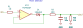
\includegraphics{img/peak_detector.pdf}
	\caption{Przykładowy schemat połówkowego detektora szczytowego}
	\label{fig:peak-detector-schematic}
\end{figure}

\subsection{Element sprzężający}
Wymagany jest układ umożliwiający tłumienie sygnału zmiennego względem sygnału sterującego:

\begin{equation}
	V_{wyj} \propto \frac{V_{wej}}{V_{ster}}
	\label{eq:coupling_1}
\end{equation}

Fizyczna implementacja takiego układu okazuje się być niebanalna.
Możlwy jest układ realizujący operacje mnożenia wartości syngałów. 
Jego realizacja jednka jest wysoce złożona i wymaga relatywnie dużo części, 
ponieważ w jego skład wchodzą układy wyznaczające logarytm natrualny obu wartości, dodające te wartości do siebie,
a na koniec wyznaczające funkcje wykładniczą $e^x$ tej sumy.

Alternatywna metoda wykożystuje element zmieniający swój opór elektyczny względem jakiegoś innego czynnika.
Przykładem historycznej realizacji takiego układu jest zastosowanie niewielkiej lapmy żarowej,
której opór włukna jest wprost proporcjonalny do jego temperatury.

Istnieje jednak znacznie prostrze i wydajniejsze rozwiązanie.

Popularnym elementem o zmiennm oporze jest fotorezystor. W przeciwieństwie do innych elementów
światłoczułych, przy stałym natężeniu światła, zachowuje się on jak faktyczny rezystor,
tzn. prąd przepływający jest wprost proporcjonalny do napięcia i odwrotnie do jego oporu
$I \propto \frac{V}{R_{\phi}}$.

Tak więc, jeśli zamknie się fotorezystor w obudowie światłoszczelnej wraz z diodą LED,
uzyskamy układ o zmiennym oporze elektrycznym, kontorlowany przez prąd diody.

\begin{equation}
	R \propto \frac{1}{I_{Led}}
\end{equation}

Umożliwia to łatwą implementacje układu sprzężenia (Eq. \ref{eq:coupling_1}). 

Co prawda powyższy model ignoruje fakt,
iż tak na prawdę opór fotorezystora zależny jest wykładniczo od natężenia padającego światła
$R = \left(\frac{1}{\phi}\right)^A$. Nie stanowi jednak to dużego problemu ponieważ układ ten znajduje się w 
pęntli sprzężenia zwrotnego.

\begin{equation}
	R \propto \frac{1}{(I_{Led})^A}
\end{equation}

\subsection{Układ odniesienia}
W tym momęcie potrzebne jest jedynie stabline oraz dostrajalne źródło napięcia odniesienia.
Do tego celu z zupełności wystarczy układ LM4041 wraz z prezcyzyjnym potencjometrem.

\section{Implementacja}

\subsection{Kod źródłowy}

\begin{figure}
	\inputminted{asm}{../src/main.S}
\end{figure}

\newpage
\printbibliography %Prints bibliography

\newpage

\begin{figure}
	\centering
	\includegraphics[width=0.75\textwidth]{img/kot_enter.jpg}
	\caption{Kot autora wspomagający proces twórczy}
\end{figure}

\end{document}